% Session 10 -- Hamiltonian learning: the forward arrow of the whole course, its inverse, and
% Placement: sec. "Hamiltonian learning", after equation (10.12).
% Rendered by figures/blender/s10f06_hamiltonianlearning.py, labels in figures/overlays/s10f06_hamiltonianlearning.tex.
\begin{aqmfigure}{fig:s10:hamlearning}{Hamiltonian learning, and why it closes the loop of the
course instead of going outside it. \textbf{Top.} The forward arrow $H\mapsto\mathcal{O}$ of (10.11)
is what sessions 1 to 9 built during all their time. The arrow that an experiment needs goes in the
other direction, and there is no closed-form inversion of it. \textbf{(a)} The solution to the lack
of experimental training data is to produce the data. We simulate $\mathcal{O}$ from many
\emph{known} Hamiltonians, so that every training pair comes with its answer $\lambda_n$ by
construction, and we fit the network with (10.12). \textbf{(b)} Only after this step the trained
network is applied to a real measurement. Note what the training set is made of, which is the
forward methods of the whole course, run many times. The final method of the course and its first
method are the same method, applied in opposite directions.}
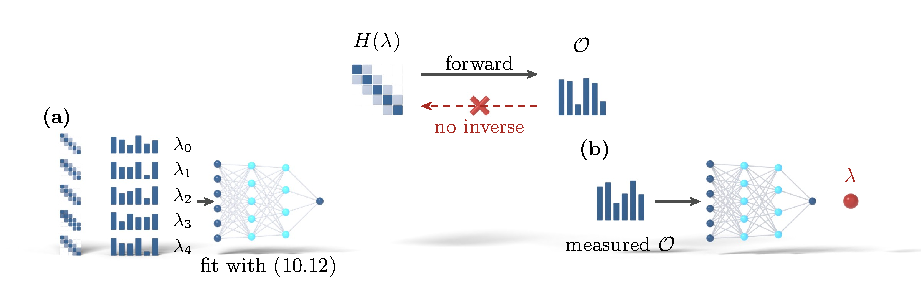
\includegraphics{figures/pdf/s10f06_hamiltonianlearning.pdf}
\end{aqmfigure}
